\section{Use cases}

\subsection{TaskDo}

TaskDo \citep{taskdo} is a task manager application written using CoffeeScript \citep{coffeescript}, Spine \citep{spinejs} and Atmosphere. It features offline usage, synchronization with Google Tasks API \citep{google_tasks} and is bundled as application for Mac platform using MacGap. \citep{macgap}

The strong point of TaskDo is its close resemblance to native application. It's bundled as one, it's very responsive, but the most imporant thing is that it uses local data, which are synced with Google Tasks API using Atmosphere.

\begin{figure}[htbp]
  \centering
    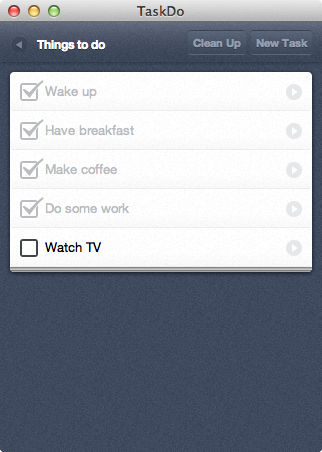
\includegraphics[height=3in]{TaskDo.png}
  \caption{Screenshot of TaskDo}
  \label{fig:taskdo}
\end{figure}

One of the problems during implementation was OAuth authentication. To successfuly authenticate user, the OAuth2 protocol \citep{oauth} first requires redirection to provider's website. Then the user has to confirm that they want to share their application data with third party application. At the end of the authentication process the user is redirected back to the original application.

\begin{figure}[ht!]
  \centering
    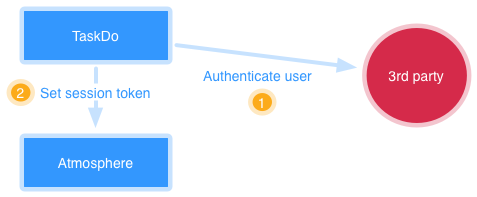
\includegraphics[width=3.5in]{TaskDoDiagram.png}
  \caption{caption}
  \label{fig:taskdo_diagram}
\end{figure}

Now the application is sent a session token, which has to be used with every subsequent API call in form of HTTP header.

Atmosphere provides a method for sending custom HTTP header with each request. TaskDo implements logic for completing the authentication process and then updates configuration for resource client to use the newly retrieved token with each request.

The Google Tasks API also returns JSON in a slightly more complicated format. For this reason, Atmoshere allows configuration of the way data are extracted from the response.

\subsection{Edukit}

